%! Date = 4/23/25
\section{Motivation}\label{sec:motivation}
\subsection{Synchronous Communication and Stragglers}\label{sec:synchronous-communication-and-stragglers}
\begin{figure}[!ht]
    \centering
    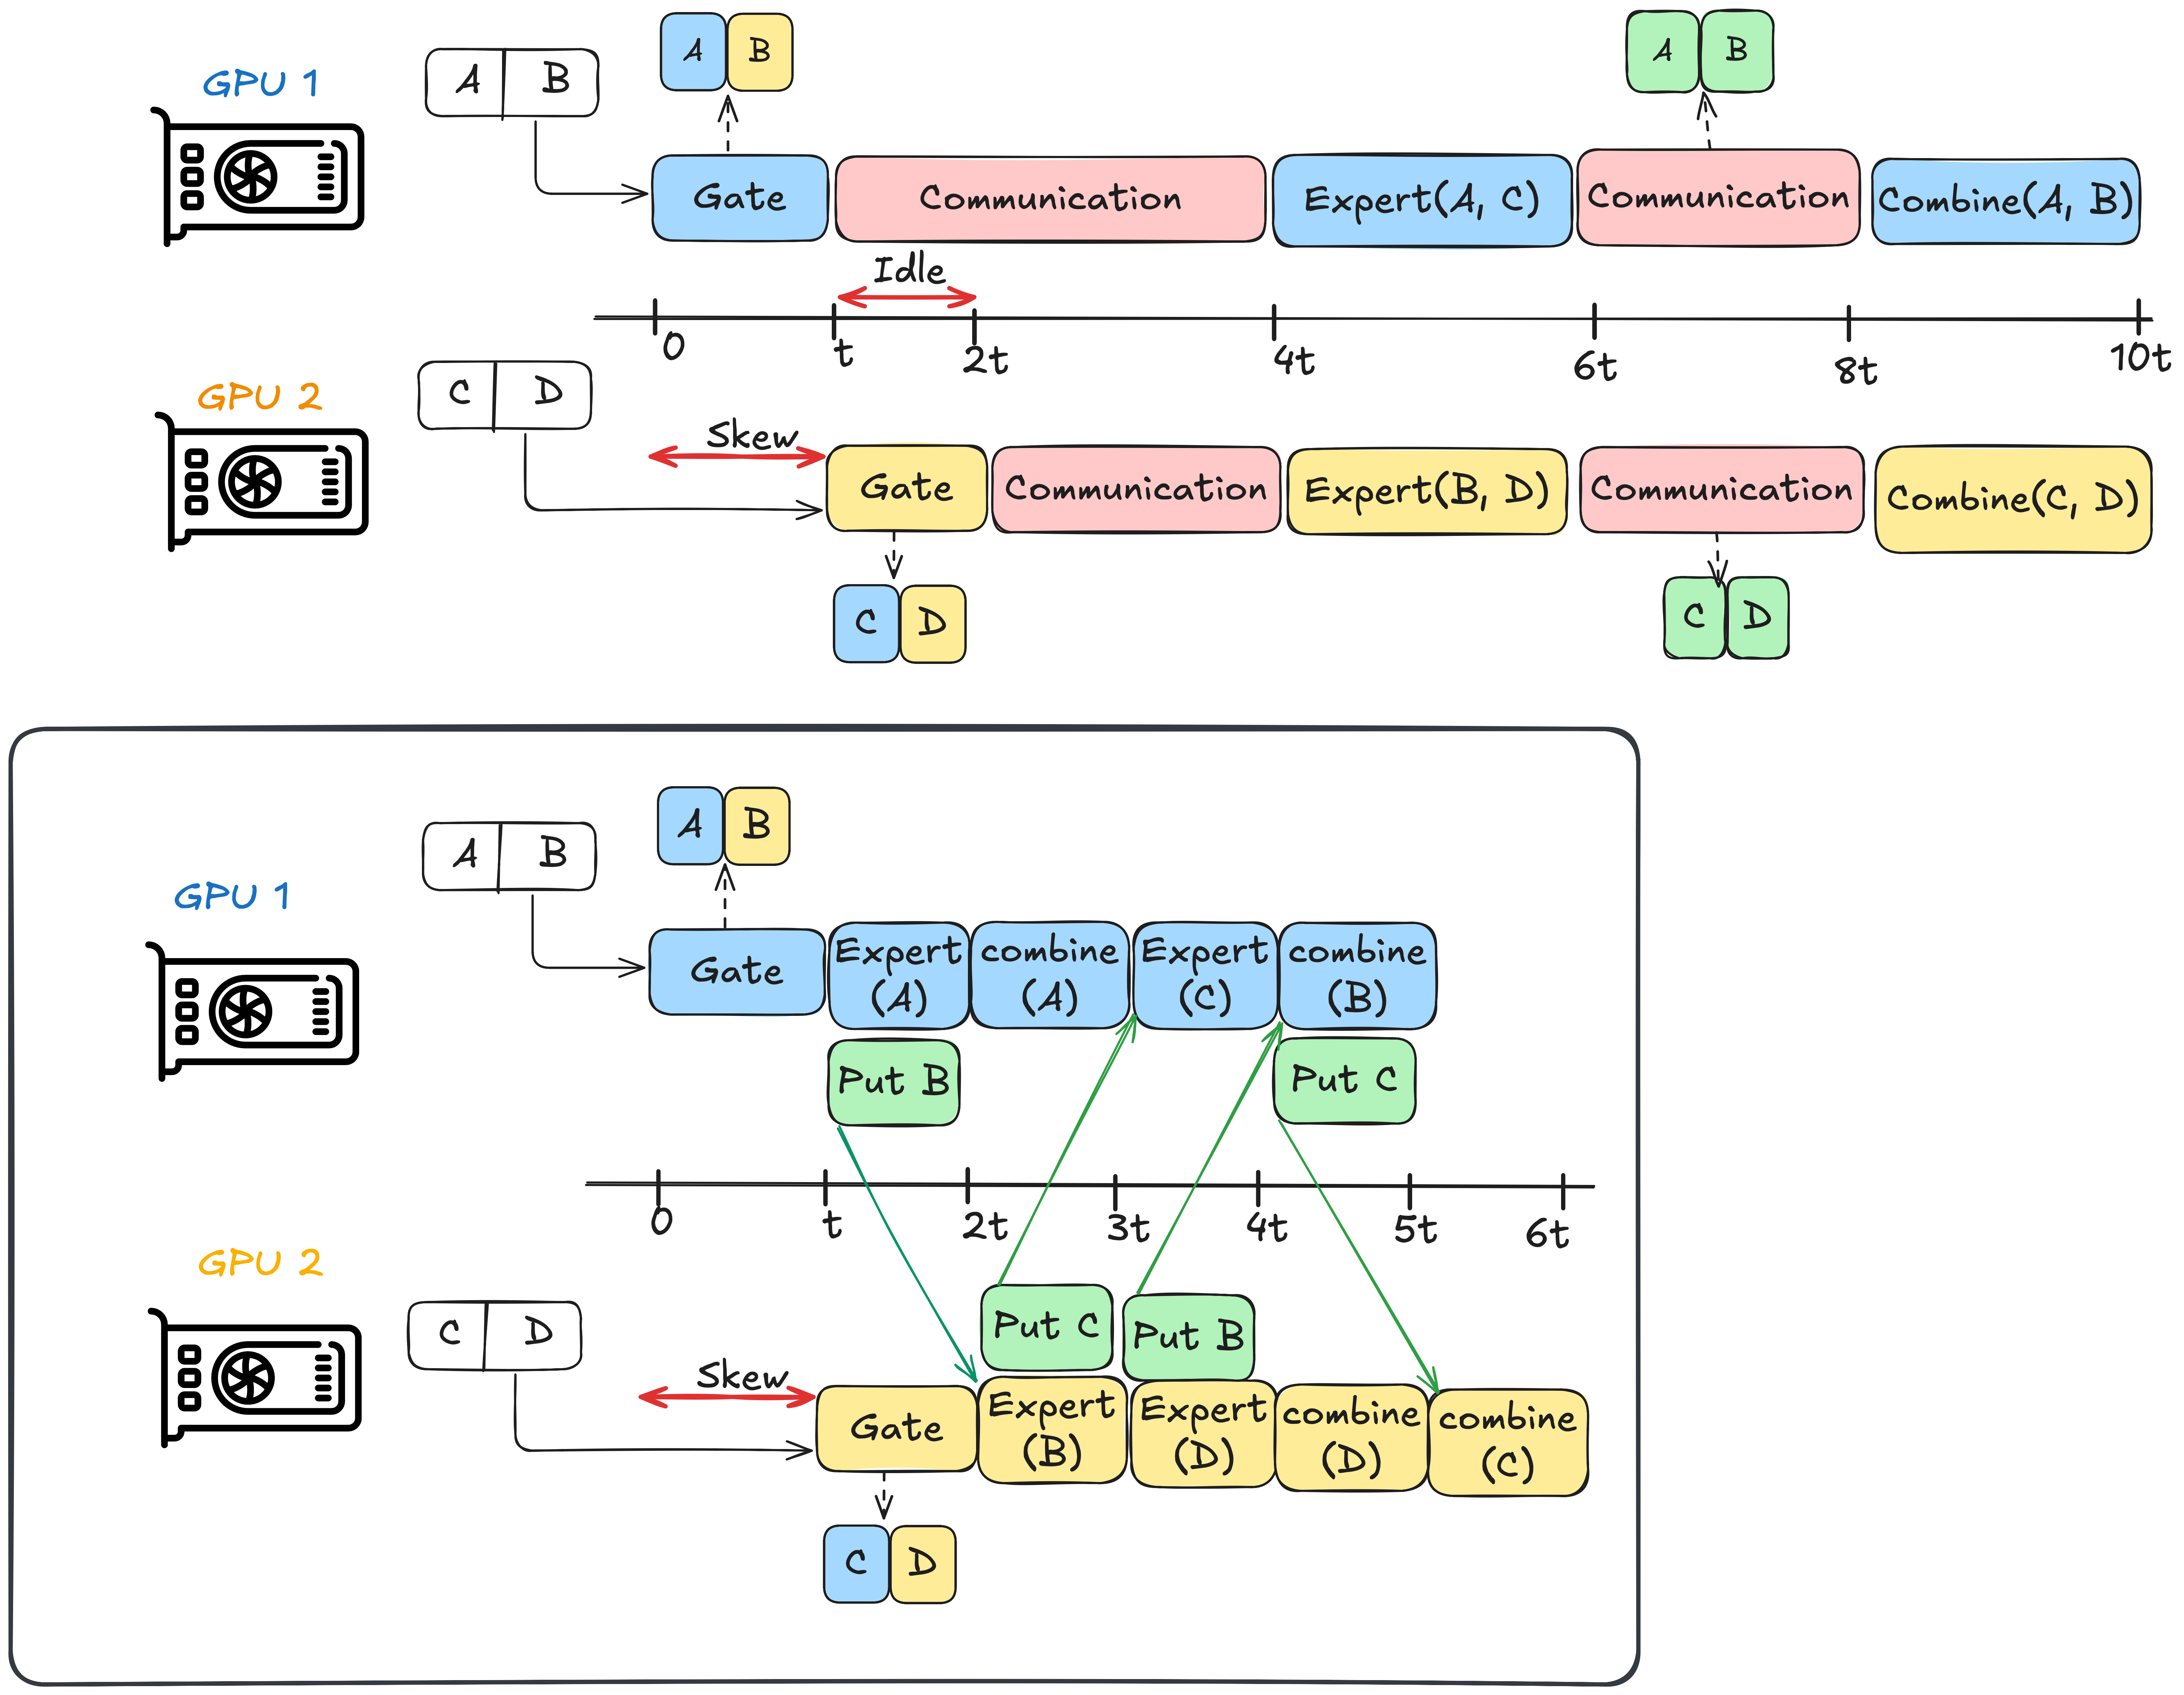
\includegraphics[width=0.8\textwidth, keepaspectratio]{figures/s_overlap}
    \caption{Overlapped Schedule (bottom) showing how idle time from the sequential schedule (top)
        is repurposed for computation. \sysname implements the overlapped schedule.}
    \label{fig:overlap}
\end{figure}
\emph{AlltoAll} or \emph{AllGather} communication as currently used in MoE frameworks
is a \emph{synchronous} collective operation, whose completion requires the participation of all involved GPUs.
Here, disparities in processing speeds or kernel scheduling
among GPUs induce a straggler effect detrimental (Figure~\ref{fig:overlap}) to (1) the collective operation's performance and (2)
E2E performance, as stalled GPUs cannot proceed to downstream dependent or independent tasks until the collective terminates.
Specifically, as shown in Figure~\ref{fig:straggler}, for distributed training of a 1.3B GPT-3 MoE model across
32 A100 GPUs, we see P95 communication performance degradation of \textbf{1.32X} when compared to the mean actual kernel time
from Figure~\ref{sub:raw_perl}.
This performance reduction is rather tame as the underlying hardware is a supercomputer well-tuned
against ``software jitter''~\cite{nerscNetworkNERSC}.
However, we observe a more severe p95 performance loss of \textbf{11X} in a single-node Virtual Machine (VM).
In line with prior HPC works~\cite{1639320, 10.1145/3545008.3545056},
we argue that obviating the inherent barrier in this synchronous collective communication would
allow GPUs to repurpose this observed idle time for downstream computation as depicted in Figure~\ref{fig:overlap}.
\begin{table}[!h]
    \centering
    \caption{Straggler Delay within Synchronous \emph{All-to-All} communication.
    We capture the distribution of delay induced by stragglers across many steps.
    Let \textbf{Actual Time} $t_a$ denote the fastest kernel execution time across all GPUs,
        and \textbf{Total Time} $t$ be the maximum recorded step time. We define
        $Delay$ as the maximum difference between $t$ and $t_a$. Note $Delay$ is idle time. For the
        1x8 V100, we profile 1750 steps and 600 steps for the 8x4 A100. See Figure~\ref{fig:straggler}
        for the raw distribution.}
    \label{tab:s_delays}
    \begin{tabular}{@{}lcccc@{}}
        \toprule
        \textbf{System}      & \multicolumn{1}{l}{\textbf{\# Nodes}} & \multicolumn{1}{l}{\textbf{\# GPUs}} & \textbf{Median} & \textbf{p95} \\ \midrule
        Commercial VM (V100) & 1                                     & 8                                    & 3.1x            & 11.4x        \\
        Supercomputer (A100) & 8                                     & 32                                   & 1.09x           & 1.32x        \\ \bottomrule
    \end{tabular}
\end{table}
\subsection{Kernel launch overhead.}\label{subsec:kernel-launch-overhead.}
\begin{figure}[!h]
    \centering
    \begin{subfigure}{0.425\textwidth}
        \centering
        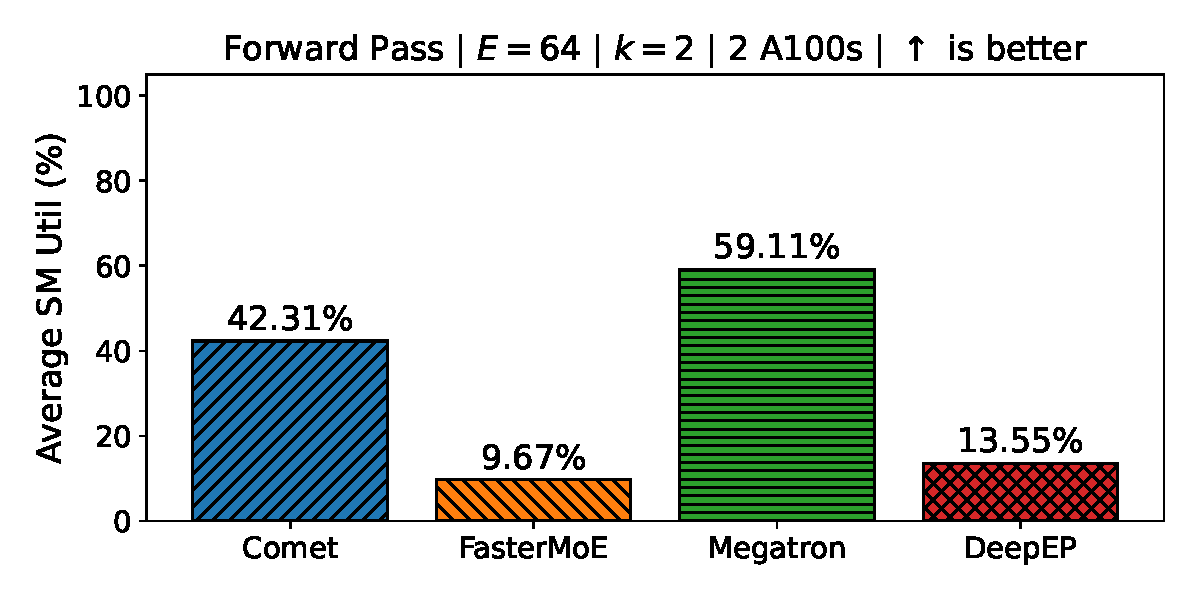
\includegraphics[width=\linewidth, keepaspectratio]{figures/sm_util_b}
        \caption{GPU SM Utilization across baselines}
        \label{sub:util}
    \end{subfigure}
    \begin{subfigure}{0.425\textwidth}
        \centering
        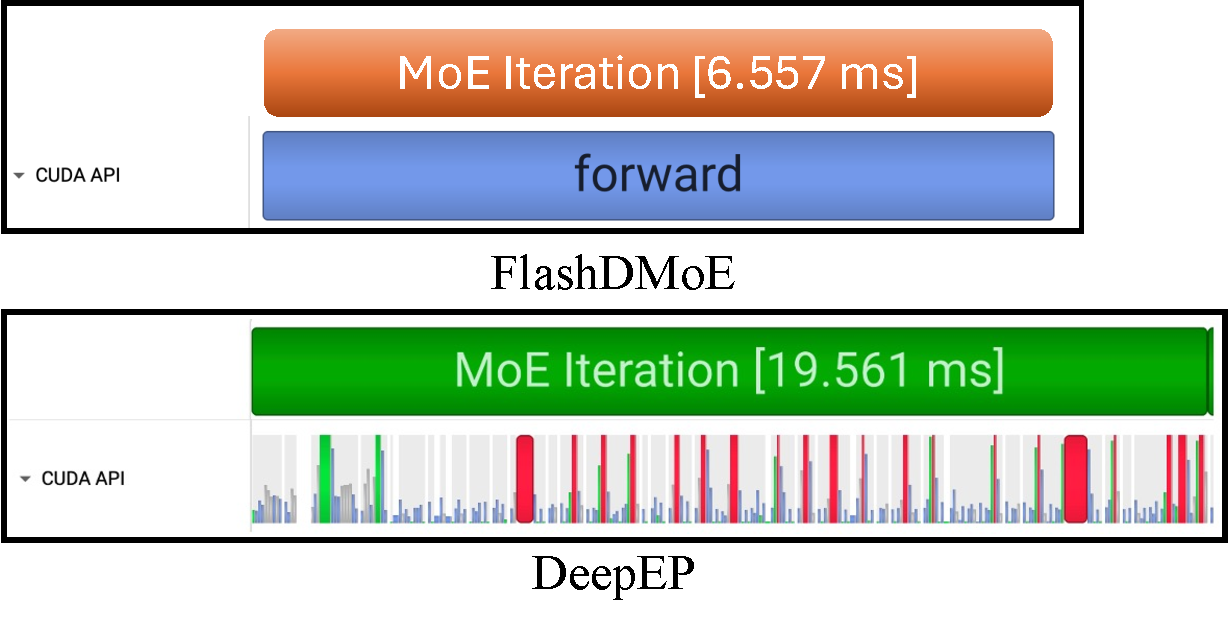
\includegraphics[width=\textwidth, keepaspectratio]{figures/kernel_launch}
        \caption{Kernel Launch overhead (CUDA API row)}
        \label{sub:launch}
    \end{subfigure}
    \caption{\ref{sub:util} shows GPU utilization averaged across 100 MoE forward passes on 2 NVLinked A100s with
    300 GB/s unidrectional bandwidth.
    Despite the high-bandwidth interconnect, we observe up to 90\% idle time,
        which we attribute to kernel launch gaps and non-overlapping communication.}
    \label{fig:kl}
\end{figure}
We compare the kernel launch overheads between \sysname and existing baselines.
Table~\ref{tab:gpuOps} shows the number of kernel launches during a single forward pass: \sysname launches exactly one persistent kernel, while the baselines launch up to 550 short-lived kernels to perform the same computation.
Figure~\ref{fig:kl} provides a visual comparison using CUDA API traces captured by NSight Systems, illustrating the difference between \sysname and DeepEP.
DeepEP exhibits numerous small CUDA API calls, with frequent stalls between individual operators, leading to increased GPU idle time (Figure~\ref{sub:util}).
In contrast, \sysname maintains high GPU utilization by avoiding launch overhead and synchronization gaps—achieving \textbf{93.17}\% GPU utilization compared to 14\% for DeepEP.
See \S\ref{sec:evaluation} for experimental results and \S\ref{sec:related} for a discussion of related work.